\documentclass{article}
\usepackage[a4paper]{geometry}
\usepackage{fancyhdr} 
\usepackage{tikz}
\usepackage{amsmath}
\usepackage{hyperref} 
\pagestyle{fancy}
\lhead{Abstände zwischen Punkten und Ebenen}
\rhead{Juli 2025}
\begin{document}
   
\newcommand{\norm}[1]{\big| {#1} \big|}  
\newcommand{\vect}[1]{\overrightarrow{#1}} 
\newcommand{\vectp}[1]{\vect{\mathrm{#1}}}
  
\section{Abstände zwischen Punkten und Ebenen}
 
\begin{minipage}[t]{\dimexpr\textwidth-5cm}
 Die einfachste Methode den Abstand zwischen einem Punkt und einer Ebene zu finden, ist das \emph{Lotfußpunktverfahren}. Dabei wird ein \emph{Lotfußpunkt} $\mathrm{F}$ bestimmt, welcher der zu $\mathrm{A}$ näheste, auf $\mathrm{E}$ liegende, Punkt ist. Die Länge des Verbindungsvektors $\vectp{PF}$ stellt nun den Abstand von $\mathrm{A}$ zu $\mathrm{E}$ dar. Somit ist der Abstand
 \[
  d(\mathrm{A}, \mathrm{E}) = \norm{\vectp{PF}}
 \] 
 Weil $\mathrm{F}$ in der Regel nicht in der Aufgabe gegeben ist, muss dieser Punkt erstmal gefunden werden. Dies wird getan, indem \\[-0.7em]
\end{minipage} 
\hfill
\begin{minipage}[t]{5cm}
 \centering 
 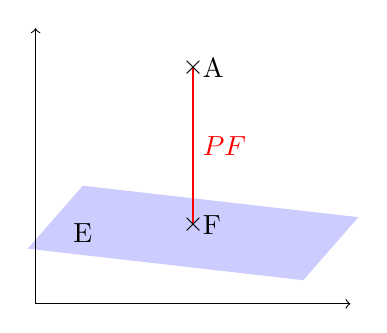
\begin{tikzpicture}[baseline=(current bounding box.north)] 
  \fill[blue!20] (-0.1, 0.7) -- (0.6, 1.5) -- (4.1,1.1) -- (3.4, 0.3) -- cycle;
  \draw (0.6, 0.9) node[black] {$\mathrm{E}$};
 
  \draw[thick,red] (2, 1) -- (2,3);
  \draw (2, 2) node[red, right] {$\vectp{PF}$}; 
  \draw (2, 3) node[black] {$\times$} node[right] {$\mathrm{A}$};  
  \draw (2, 1) node[black] {$\times$} node[right] {$\mathrm{F}$};
  \draw[->] (0, 0) -- (4, 0); 
  \draw[->] (0, 0) -- (0, 3.5);
 \end{tikzpicture}
\end{minipage}
eine Gerade, genannt die \emph{Lotgerade}, bestimmt wird, welche vom Punkt $\mathrm{A}$ aus auf direktestem Wege zur Ebene $\mathrm{E}$ geht. Offensichtlich muss die Lotgerade dafür Senkrecht zur Ebene sein, heißt kollinear zum Normalvektor $\vect{n}$. Daraus folgt die Lotgerade
\[
 g: \vect{x} = \vectp{OP} + t \cdot \vect{n} 
\]
Zusammen mit der Gleichung der Lotgerade und der Ebene kann nur deren Schnittpunkt, welcher auf der Lotfußpunkt $\mathrm{F}$ ist, gefunden werden, mithilfe dessen nun auch $\vectp{PF}$ und somit $\norm{\vectp{PF}}$ bestimmt werden kann.
 
Muss der Aufgabe nach $\mathrm{F}$ aber nicht angegeben werden, können die letzten wenigen Schritte aber auch übersprungen werden und 
\(
 d(\mathrm{A}, \mathrm{E}) = \norm{t} \cdot \norm{\vect{n}}
\)
genutzt werden. Dies folgt aus 
\begin{align*}
 d(\mathrm{A}, \mathrm{E}) &= \norm{\vectp{AF}} \\
  &= \norm{\vectp{OA} - \vectp{OF}} \\ 
  &= \norm{\vectp{OA} - (\vectp{OA} + t \cdot \vect{n})} \\
  &= \norm{t \cdot \vect{n}} \\
  &= \norm{t} \cdot \norm{\vect{n}}
\end{align*}
 
\noindent \begin{minipage}[t]{\dimexpr\textwidth-8cm} 
 \subsection{Hesse'sche Normalform}
 Hat die Ebene einen Stützpunkt $\mathrm{P}$, so kann ein rechtwinkliges Dreieck zwischen $\mathrm{P}$, $\mathrm{A}$ und einem Punkt der gleichen Distanz zwischen $\mathrm{A}$ und $\mathrm{E}$ von $\mathrm{P}$ entfernt gebildet werden. Wird in diesem Dreicken der Winkel $\alpha$ am Punkt $\mathrm{P}$ eingefügt, hat dieses die Ankathete $d(\mathrm{A}, \mathrm{E})$ und die Hypothenuse $\vectp{PA}$.
 Demnach gilt für $\alpha$
\end{minipage} 
\hfill
\begin{minipage}[t]{8cm} 
 \centering 
 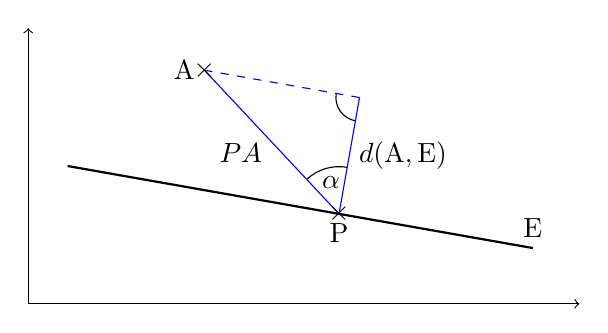
\begin{tikzpicture}[baseline=(current bounding box.north)]
  \coordinate (start) at (0.5,1.75);
  \path (start) ++({sin(100)*6}, {cos(100)*6}) coordinate (end);
  \path (start) ++({sin(100)*3.5}, {cos(100)*3.5}) coordinate (mid);
  \path (mid) ++({sin(10)*1.5}, {cos(10)*1.5}) coordinate (middist);
  \path (middist) ++({sin(-80)*2}, {cos(-80)*2}) coordinate (pointa);
  
  \draw (mid) ++({sin(10)*0.6}, {cos(10)*0.6}) arc[start angle=80, end angle=132, radius=0.6];
  \draw (middist) ++({sin(-80)*0.3}, {cos(-80)*0.3}) arc[start angle=170, end angle=260, radius=0.3];
  
  \draw[thick, black] (start) -- (end) node[above, black] {$\mathrm{E}$};
  \draw[blue] (mid) -- (middist) node[midway, right, black] {$d(\mathrm{A},\mathrm{E})$};  
  \draw[dashed, blue] (middist) -- (pointa) node[left, black] {$\mathrm{A}$};  
  \draw[blue] (mid) -- (pointa) node[midway, left, yshift=-4pt, black] {$\vectp{PA}$};
 
  \draw (mid) ++ (-0.1, 0.4) node[black] {$\alpha$};
 
  \draw (mid) node[below] {$\mathrm{P}$};  
  \draw (pointa) node {$\times$};  
  \draw (mid) node {$\times$};
 
  \draw[->] (0, 0) -- (7, 0); 
  \draw[->] (0, 0) -- (0, 3.5);
 \end{tikzpicture}   
\end{minipage} 
 
\allowdisplaybreaks 
\begin{align*} 
 \cos(\alpha) &= \frac{d(\mathrm{A}, \mathrm{E})}{\norm{\vectp{PA}}}
 && \vert\, \text{Nach Distanz Umformen} \\
 d(\mathrm{A}, \mathrm{E}) &= \cos(\alpha) \cdot \norm{\vectp{PA}} 
 && \vert\, \text{\hyperref[Winkel]{$\cos(\alpha)$ durch das Skalarprodukt ausdrücken}} \\
 &= \frac{\vect{n} \cdot \vectp{PA}}{\norm{\vect{n}} \cdot \norm{\vectp{PA}}} \cdot \norm{\vectp{PA}} \\
 &= \frac{1}{\norm{\vect{n}}} \cdot \vect{n} \cdot \vectp{PA}
 && \vert\, \text{$\vectp{PA}$ in $\vectp{OA}-\vectp{OP}$ aufspalten} \\
 &= \frac{1}{\norm{\vect{n}}} \cdot \left(\vect{n} \cdot \vectp{OA} - \vect{n} \cdot \vectp{OP}\right)
\end{align*} 
Weil das Ergebniss bei bestimmten Winkeln negativ sein kann, welches im Kontext von Abständen aber keinen Sinn ergibt, wird die Formel in den Betrag gesetzt. Somit gilt
\[
 d(\mathrm{A}, \mathrm{E}) = \frac{1}{\norm{\vect{n}}} \cdot \norm{\vect{n} \cdot \vectp{OA} - \vect{n} \cdot \vectp{OP}} 
\] 
Offensichtlich ist ein jeder Punkt $\vect{x}$, welcher keinen Abstand zur Ebene hat, also für welchen $d(\mathrm{A}, \mathrm{E})=0$ gilt, ein Punkt auf der Ebene  
\[
 \frac{1}{|\vect{n}|} (\vect{n} \cdot \vect{x} - \vect{n} \cdot \vectp{OP}) = 0 
\] 
 
\subsection{Abstände zwischen Punkten und Geraden}
\begin{minipage}[t]{\dimexpr\textwidth-5cm}  
Der Abstand zwischen einem Punkt P und einer Gerade $g$, $d(\text{P}, g)$, kann berechnet werden, indem der Punkt F der Gerade gefunden wird, welcher den geringsten Abstand zu P hat und der Abstand zwischen den Punkten P und F berechnet wird.
Dabei ist Auffällig, dass zwischen dem Verbindungsvektor $\vectp{PF}$ und der Gerade $g$ (beziehungsweise dessen Richtungsvektor $\vect{u}$) ein rechter Winkel liegt, heißt, sie sind kollinear. Es gilt
\[
 d(\text{P}, g) = \norm{\vectp{PF}} \quad \text{mit} \quad \vectp{PF} \cdot \vect{v} = 0
\]
Dabei ist der Punkt F natürlich ein Punkt der Gerade $g$, liegt also in der generellen Geradengleichung, ist also einer der Punkte $\vectp{OX}_r$ mit
\end{minipage}
\hfill
\begin{minipage}[t]{5cm}
 \centering 
 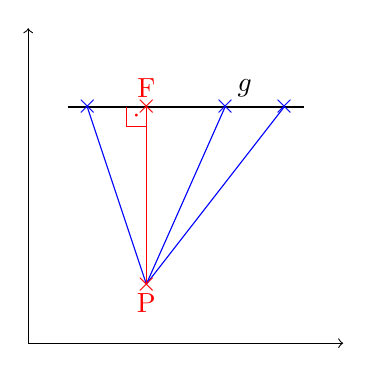
\begin{tikzpicture}[baseline=(current bounding box.north)]
  \coordinate (start) at (0.5,1.75);
  
  \draw (0.5, 3) -- (3.5, 3) node[pos=0.75, above]{$g$};  
  \draw[blue] (1.5, 0.75) -- (0.75, 3) node{$\times$};
  \draw[blue] (1.5, 0.75) -- (2.5, 3) node{$\times$};
  \draw[blue] (1.5, 0.75) -- (3.25, 3) node{$\times$}; 
  \draw[red] (1.5, 0.75) -- (1.5, 3) node[pos=0]{$\times$} node[pos=0, below]{P} node[pos=1]{$\times$} node[pos=1, above]{F};
  \draw[red] (1.25, 3) -- (1.25, 2.75);
  \draw[red] (1.25, 2.75) -- (1.5, 2.75);
  \draw[red] (1.5 - 0.125, 3 - 0.125) node{$\cdot $};  
 
  \draw[->] (0, 0) -- (4, 0); 
  \draw[->] (0, 0) -- (0, 4);
 \end{tikzpicture}    
\end{minipage} 
\[
 \vectp{OX}_r = \vectp{OA} + r \cdot \vect{u} 
\]
Wird hier $\vectp{OP}$ abgezogen gilt nach $\vectp{AX}_r = \vectp{OX} - \vectp{OP}$ für ein jedes $r$ der Verbindungsvektor zum Punkt P
\[
 \vectp{PX}_r = \vectp{OA} + r \cdot \vect{u} - \vectp{OP}
\]
Nun muss nach dem $r$ aufgeläst werden, für welches die obige Kollinearität gegeben ist, weil dieses $r$ auch dasselbe $r$ des Punktes F ist. 
\[
 (\vectp{OA} + r \cdot \vect{u} - \vectp{OP}) \cdot \vect{v} = 0
\]
Das gefundene $r$ kann in die obigen Formeln eingesetzt werden um den Punkt F und die Distanz $\norm{\vectp{PF}}$ zu finden.
 
\subsection{Abstände zwischen zwei Geraden}
Sind zwei Geraden identisch, schneiden sich oder sich echt parallel, ist der Abstand $d(g_1, g_2)$ trivial. 
 
Der Abstand von zwei windschiefen Geraden ist die Länge des kürzesten Verbindungsvektors von zwei Punkten der Geraden. Es ist verständlich, dass der Verbindungsvektor, wie auch oben, zu beiden Geraden orthogonal sein muss.
\[
 \vect{c} = \vectp{X}_s - \vectp{X}_r 
\]  
Es wird der Verbindungsvektor gebildet, indem die Punkte der Geraden in Abhängigkeit von dem jeweiligen Parameter gefunden und subtrahiert wird. Es folgt eine Formel für den Verbindungsvektor, welche von zwei Parametern abhängig ist. Es wird jeweils das Skalarprodukt von diesem Verbindungsvektor und den Richtungsvektoren gleich null gesetzt.
\[
 \vect{c} \cdot \vect{v} = 0
 \quad \text{und} \quad
 \vect{c} \cdot \vect{u} = 0
\] 
Diese beiden Gleichungen können nach den Parametern der Geraden, welche die beiden nähesten Punkte angeben, aufgelöst werden. Anhand der gefundenen Parameter können diese Punkte (wenn nötig) berechnet werden, der Verbindungsvektor kann gefunden werden, die Länge des Verbindungsvektors, welche auch die zu findene Distanz ist, kann bestimmt werden.
 
 
\end{document}